\documentclass[]{report}
\usepackage[utf8]{inputenc}
\usepackage[francais]{babel}
\usepackage{graphicx}

% Title Page
\title{Ghosts}
\author{Clara Bringer et Pierre Gervais}

\begin{document}
\maketitle

\section{Liste des fonctionnalités}

\paragraph{Préparation de la partie}
\subparagraph*{}
Avant que la partie ne commence, vous êtes invités a sélectionner (ou non) le mode triche puis à choisir des extensions parmi une liste.
\subparagraph*{}
Vous pouvez faire jouer automatiquement un ou deux joueurs à l'aide d'un fichier en \textit{.gf} décrivant la disposition initiale des fantômes ainsi que les déplacements que le joueur effectuera.\\
\emph{Attention : Si un joueur automatique ne peut pas placer ses pions comme décrit dans son fichier car sa disposition est incompatible avec les règles, ou si il ne peut pas effectuer un déplacement car celui-ci est illégal, une exception est lancée.}

\paragraph{Placement des fantômes}
\subparagraph*{}
En cliquant sur une case, la fenêtre propose d'y placer un fantôme en choisissant :
\begin{itemize}
	\item Son type, vous avez le choix parmi le type de fantôme "basique" et les éventuels autres types contenus dans les extensions sélectionnées
	\item S'il est bon ou mauvais
\end{itemize}
\subparagraph*{}
Vous pouvez supprimer un pion en cliquant dessus puis en confirmant la suppression.

\paragraph{Déroulement du jeu}
\subparagraph{Déplacements}
Chaque joueur doit pour déplacer ses pions cliquer sur l'un de ses fantômes, puis cliquer sur la case en surbrillance où il souhaite le déposer.
\subparagraph{Fin de jeu}
Si le livre de règles indique que la partie est terminée, le jeu annonce l'éventuel gagnant (ou match nul si c'est le cas) puis ferme le programme.

\section{Diagrammes de classe}

\begin{figure}
	\caption{Diagramme de classes du package core}
	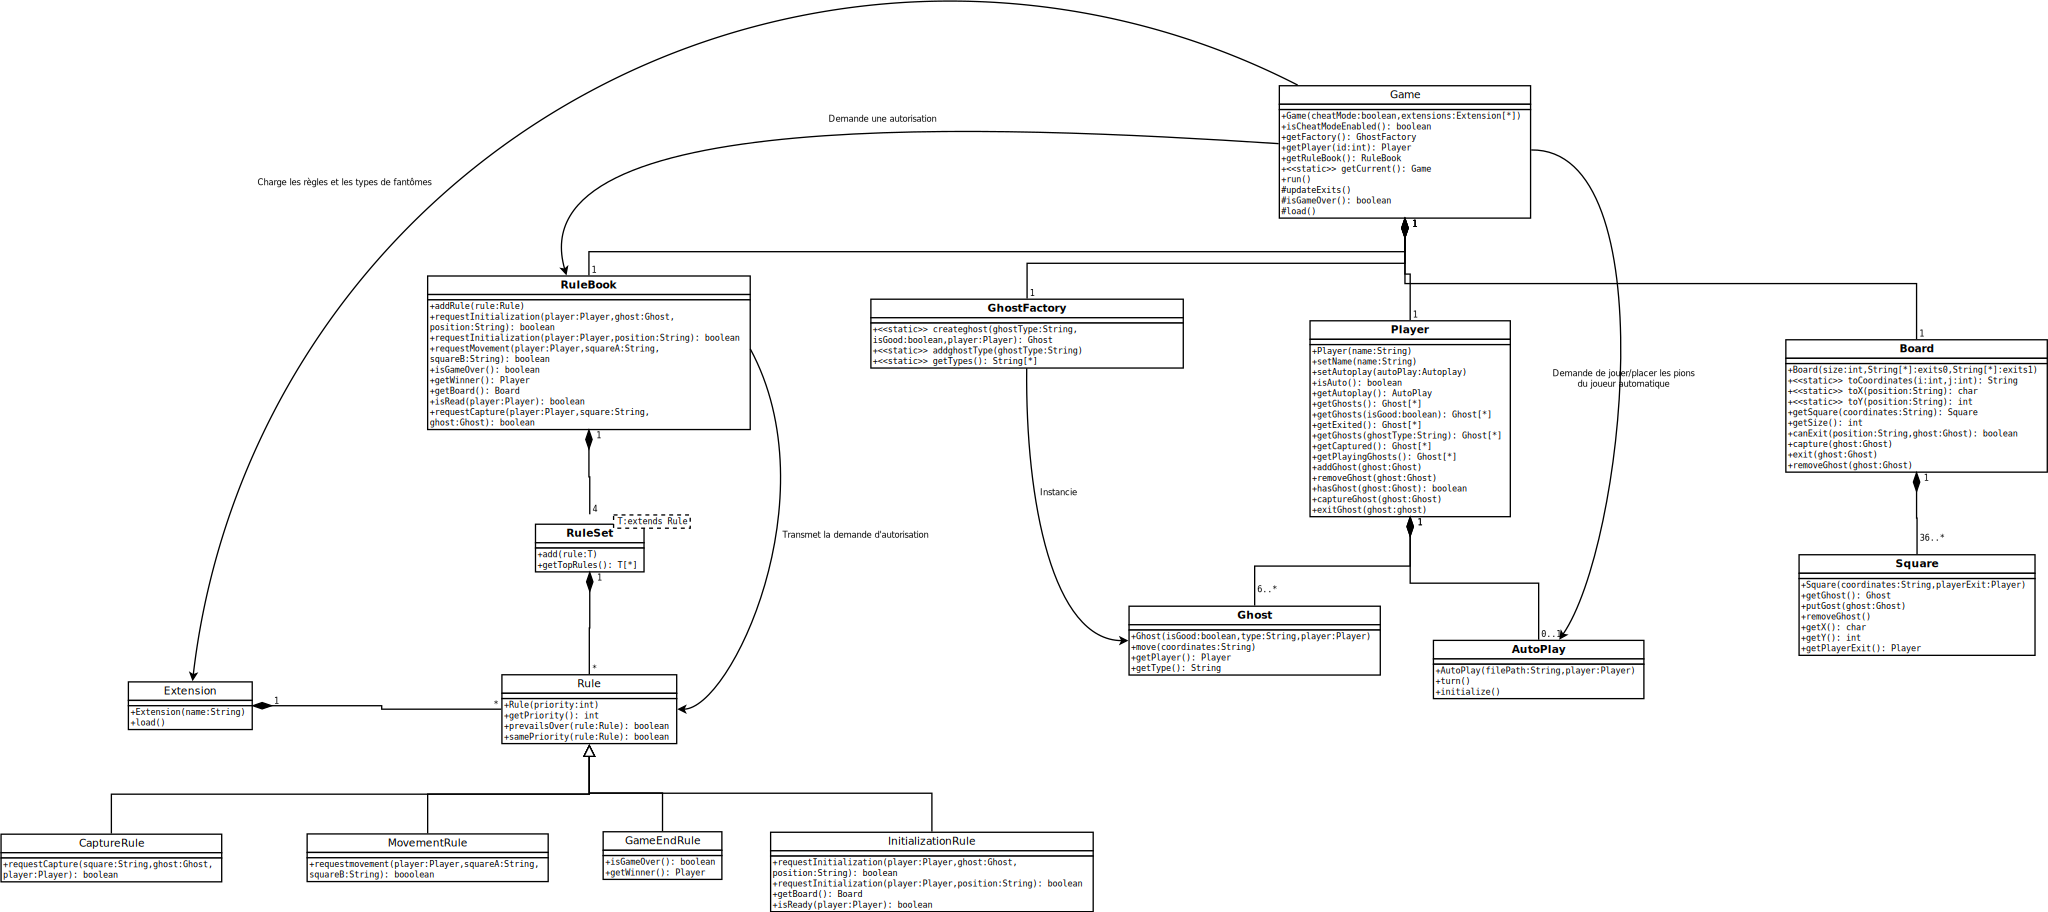
\includegraphics[width=\textwidth]{core.png}
\end{figure}

\begin{figure}
	\caption{Diagramme de classes du package core.GUIGame}
	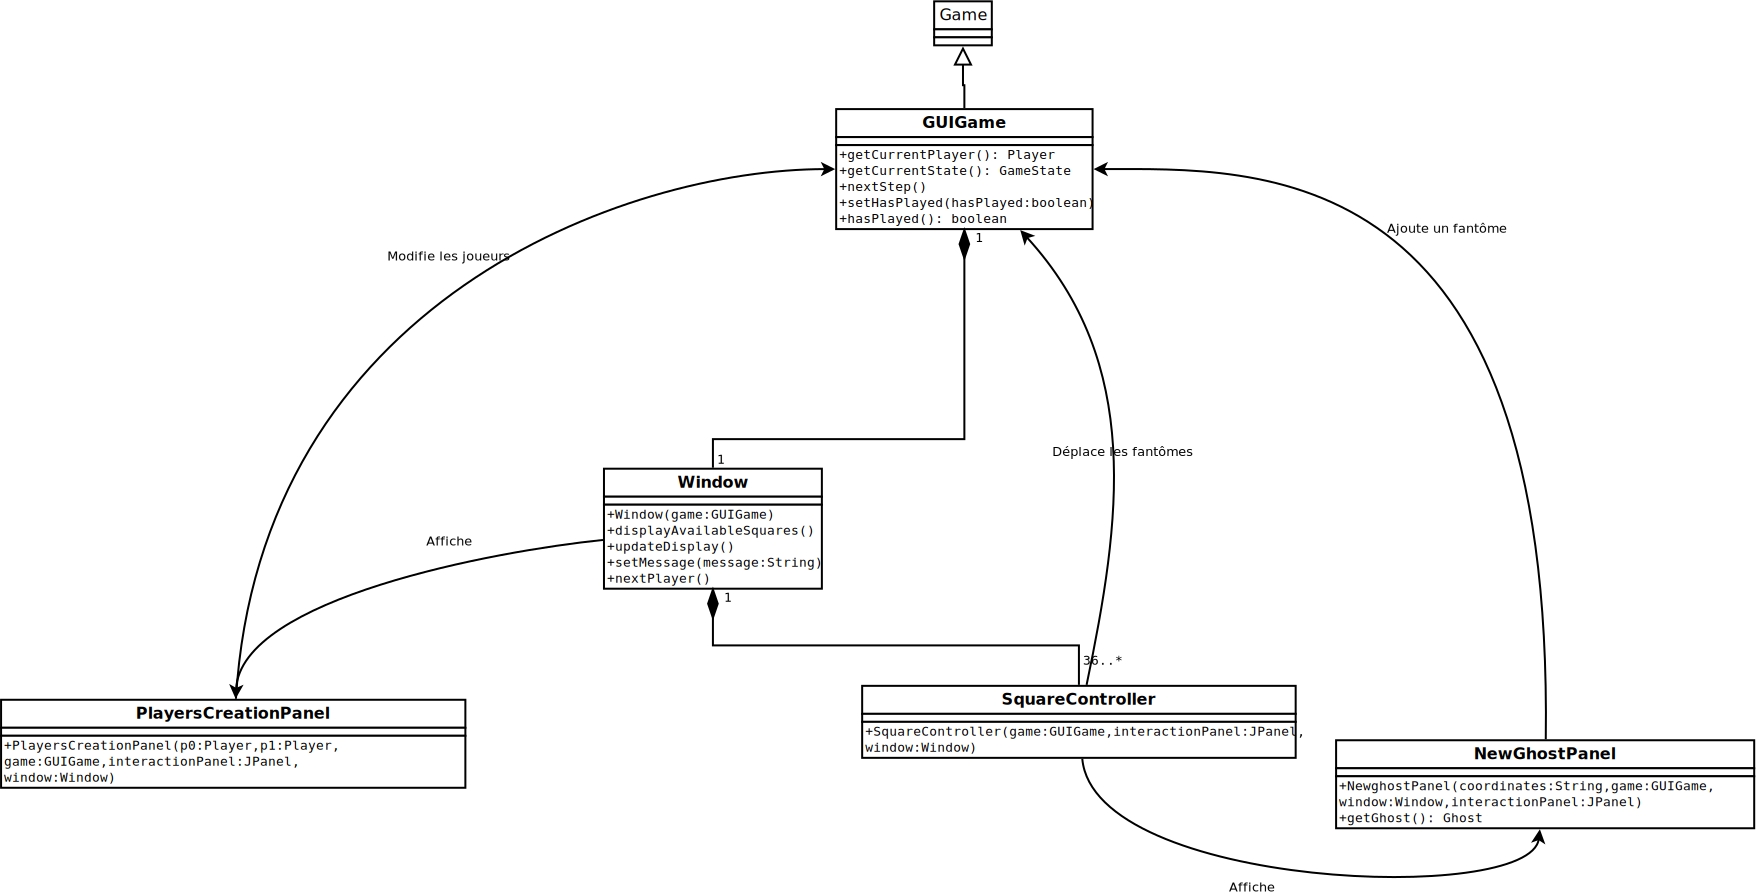
\includegraphics[width=\textwidth]{core_GUIGame.png}
\end{figure}

Les diagrammes sont disponibles depuis la doc en grand format dans la description des packages core et core.GUIGame.

\end{document}
